%!TEX encoding = UTF-8 Unicode
% !TeX spellcheck = en_GB

%%%%%%%%%%%%%%%%%%%%%%%%%%%%%%%%%%%%%%
\chapter{ Overview of Higgs production at colliders }\label{chap:overviewSingleHiggs}
%%%%%%%%%%%%%%%%%%%%%%%%%%%%%%%%%%%%%%
The four most important Higgs production processes at the LHC: gluon fusion~(ggF), vector-boson fusion~(VBF), vector bosons Higgsstrahlung~($Vh$), and the production with top (and anti-top) pair~($th / t \bar th$). It should be noted that sometimes the ggF category will include the quark anti-quark annihilation, but this is negligible in the SM but becomes important for significant modifications of light Yukawa couplings. These processes are illustrated in~\autoref{fig:singlehiggs}, and their details were summarised in~\autoref{table:singlehiggs}. These four channels have been observed at the LHC with $>5 \sigma$ significance. \\ 
This chapter aims to provide an overview of the current theoretical status of these channels.
\begin{table}[htbp!]
	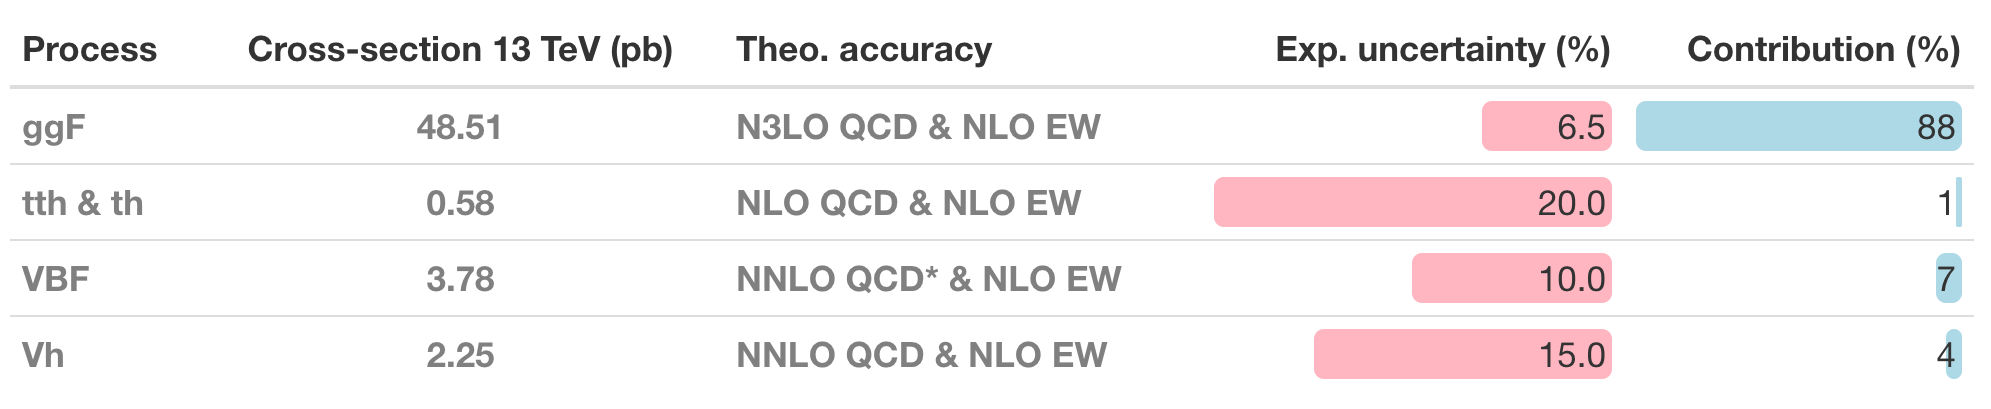
\includegraphics[width=1\textwidth]{single_higgs_table}
	\caption{ Summary of the Higgs production processes at the LHC. \label{table:singlehiggs} }
\end{table}
\begin{figure}[htbp!]
	\begin{center}
		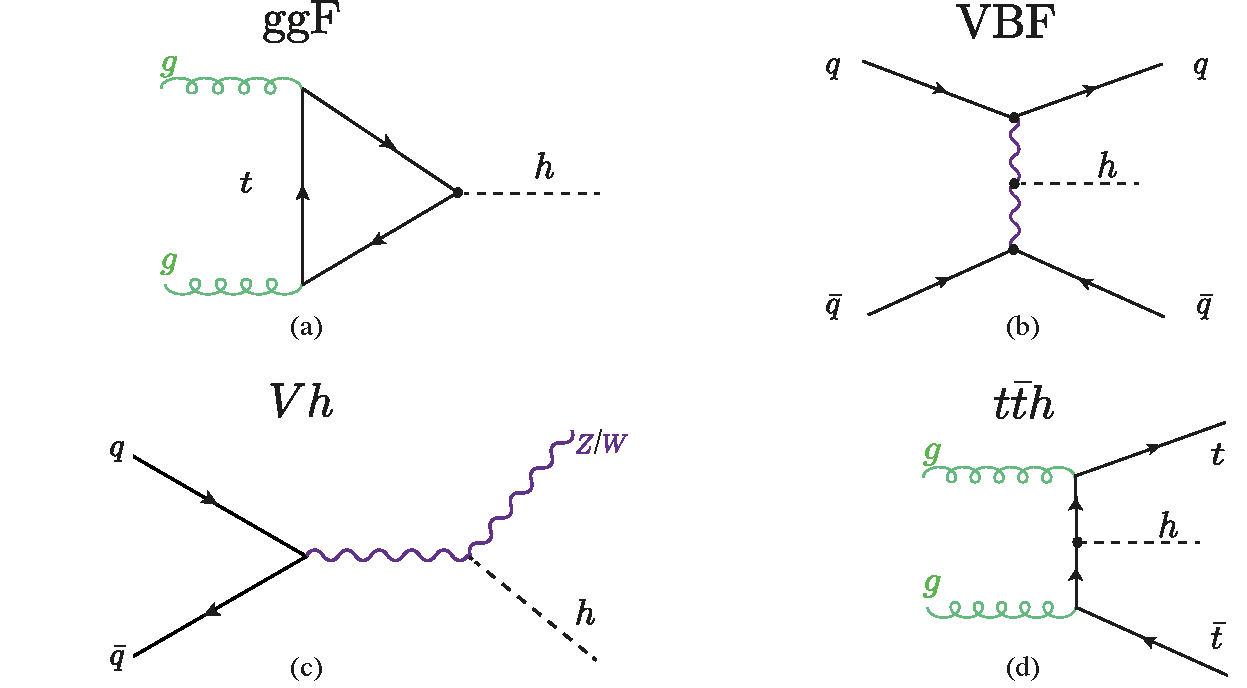
\includegraphics[width=.75\textwidth]{figures/single_higgs}
		\caption{Feynman-diagram examples of the leading Higgs production processes  at the LHC. \label{fig:singlehiggs} }
	\end{center}
\end{figure}
\section{Current status of the Higgs production channels  \label{sec:singlehiggschannels}  }
\subsection{Gluon fusion process}
The  gluon fusion~(ggf) has the largest cross-section amongst all the Higgs production channels, and consequently has the lowest experimental uncertainty. This motivates continuos improvements of its theoretical prediction.  The current state-of-the-art theoretical computation for the Higgs inclusive cross-section is N$\,^3$LO in QCD~\footnote{in the heavy top limit} and NLO in EW~\cite{Bonetti:2018ukf}. A full differential cross-section for the final state~$ gg \to h \to \gamma \gamma$ has been computed recently to~N$\,^3$LO in QCD, also for the kinematic variables~$y_h, \ y_{\gamma_1},\ y_{\gamma_2},\ \Delta y_{1,2}$ using the projection-to-born method~\cite{Chen:2021isd}. In addition, the fiducial differential cross-section in $\pt$ with experimental cuts has been computed up to third resummed logarithms~\footnote{Resummation implies accounting for a logarithmically enhanced subset of terms at each and every order of the perturbative series.} and fixed order, i.e.  N$\,^3$LL$^\prime$   N$\,^3$LO dependence~\cite{Billis:2021ecs}. \\ The state-of-the-art total theoretical uncertainty is~$5.4 \%$; this includes  uncertainties comes from the branching fraction calculation, PDF+$\alpha_s$, missing higher-order EW corrections and quark mass uncertainties. 
%\begin{figure}[htbp!]
%	\begin{center}
%		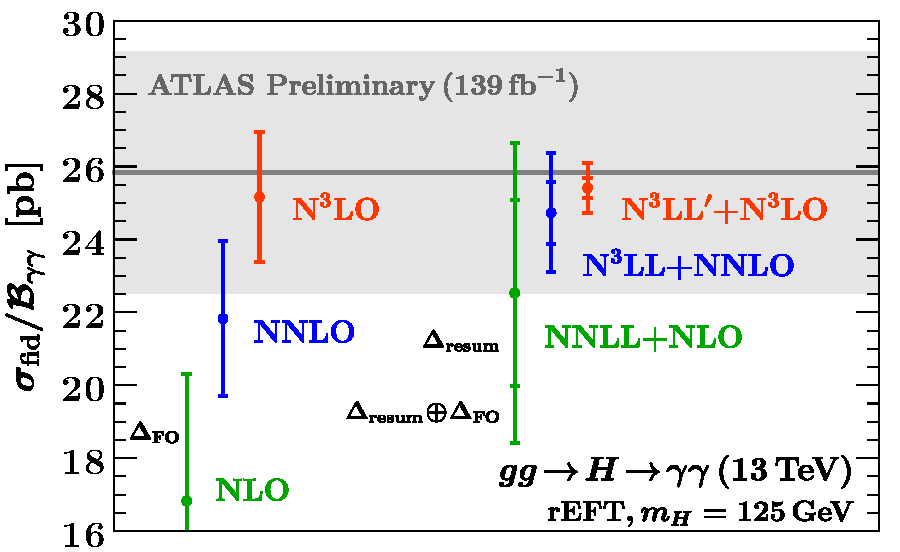
\includegraphics[width=.7\textwidth]{figures/total_xs_fid}
%		\caption{ The total fiducial cross-section for the final state  $ gg \to h \to \gamma \gamma$ at both fixed and resummed third order compared to the experimental ATLAS measurement~\cite{ATLAS:2019jst}. This figure is taken from~\cite{Billis:2021ecs}. \label{fig:ggFxs} }
%	\end{center}
%\end{figure}
The predictions can be further improved by the computation of mixed QCD-EW effects. The virtual corrections of these effects were computed in~\cite{Bonetti:2017ovy}, while the two-loop effects with two particle final states appearing in the real corrections of $ gg \to hg$  were computed in~\cite{Bonetti:2020hqh}. The computation was completed by inclusion of light quark initial states for the real corrections in~\cite{Becchetti:2020wof} with exact quark mass dependence, reducing the EW uncertainty from $2\%$ to $ \sim 0.6\%$.  \\ The computation of the three-loop form-factors with full top-mass dependence was carried out by~\cite{Czakon:2020vql,Czakon:2021yub}. However, there remains an intricate interplay between the mass effects of $gg$, $qg$ and $qq$ initial states for the real matrix elements that cannot be fully controlled due to the light quark mass effects. \\ NLO corrections to the $h +j$ and $ h+2j$ processes were computed by~\cite{Maltoni:2014eza} in the FT-approximation that uses exact born and real correction amplitudes, then approximates the two-loop virtuals by
\begin{equation}
	|	\mathcal A^{\mathrm{2-loop}}(m_t,\mu_R^2) |^2 \approx  |	\mathcal A^{\mathrm{1-loop}}(m_t\to \infty,\mu_R^2) |^2\, \frac{|	\mathcal A^{\mathrm{1-loop}}(m_t) |^2}{A^{\mathrm{(0)}}(m_t)\to \infty |^2}. 
\end{equation}
This approximation works superbly even for $ \pt \gg m_t$. Later, the full top mass effects computations have been carried out in~\cite{Kudashkin:2017skd, Lindert:2018iug} using the high energy~(HE) expiation technique. 
\subsection{Vector boson fusion}
The VBF channel has a distinctive signature, making it a\textit{ bona fide} channel for Higgs signal extraction. The suppressed colour exchange between the quarks results in a little jet activity in the central rapidity region. The quarks will be scattered into two forward jets such that the decay products of the Higgs are found in the region between them.  These features allow for excellent measurement of Higgs couplings, observation of challenging decays, and $\mathcal{CP}$ properties determination. Some of these features are also shared with the $Vh$ production channel. Both of these channels contain the $VVh$ vertex that could be written generally as~\cite{LHCHiggsCrossSectionWorkingGroup:2016ypw}
\begin{equation}
	T^{\mu \nu}(p_1,p_2) = a_1 g^{\mu \nu}+ a_2  \left(g^{\mu \nu}- 2\frac{p^\mu_{2} p^\nu }{p_1 \cdot p_2} \right)  + a_3 \frac{p_1^\alpha p_2^ \beta}{p_1 \cdot p_2}\epsilon^{\mu \nu \alpha \beta}. 
\end{equation} 
In the SM, only $a_1\neq0$, while the rest of the coefficients represent the anomalous coupling. For example, if $a_3 \neq0$, then the Higgs is  $\mathcal{CP}$ odd. The study of the azimuthal angle distribution~$d \sigma_{VBF} / d \Delta \phi_{jj}$ allows for the determination of these coefficients, with very little dependence on the higher-order perturbative corrections~\cite{hankele2006anomalous}.\\  The NLO QCD inclusive cross-section is known since the 90's~\cite{Han:1992hr}. Later, these corrections were made for the differential distributions cf.~\cite{Figy:2003nv,Berger:2004pca}. Unlike the ggF channel, which has an NLO  K-factor of $1.6$ at 13 TeV~\cite{Gomez-Bock:2007azi}, the VBF NLO corrections are small $\sim 10\%$. The two-loop NNLO QCD cross-section has been computed, and the most recent results of the two-loop computation were calculated via the structure-function approach~\cite{Bolzoni:2010xr}, in addition to STXS level 1.2 bins with EW corrections~\cite{Denner:2014cla}. These calculation are implemented in the MC event generator  \texttt{HAWK}~\cite{Ciccolini:2007jr,Denner:2011id,Denner:2014cla,Denner:2018opp}. Although these are small corrections, they are non-negligible, and their inclusion is important for uncertainty reduction.
\subsection{Associated production with EW bosons \label{vhproduction}}
The vector boson Higgsstrahlung channels $pp\to Wh/Zh$ are at tree-level processes quark-initiated  \textbf{Drell-Yan processes}~ \cite{Han:1991ia,Brein:2003wg}. They have been computed up to  NNLO in QCD ($\sim \alpha_s^2$), and  NLO EW  ($\sim \alpha^2 $)~\cite{Amoroso:2020lgh}.
%%
\par Despite arising for the first time at NLO, the gluon fusion channel $g g \rightarrow Zh$ has a non-negligible contribution to the total hadronic cross-section~$pp\to Zh$ that reaches up to $16\%$ of the total cross-section contribution at $14$ TeV~\cite{Cepeda:2019klc}, see~\autoref{fig:hzratio}. The contribution becomes more significant when one considers the  large invariant mass bins of the differential cross-section. Because at large $x$ gluons are relatively more abundant at the LHC and the extra enhancement coming from the top quark initiated contribution near the~$t\bar t$ threshold~\cite{Englert:2013vua}, also it has a higher scale uncertainty than the quark anti-quark annihilation~$\qqA$ channel. Leading to a higher theoretical uncertainty of the $Zh$ channel with respect to $Wh$, where no gluon fusion channel is present. This highlights the need to calculate the~$g g \rightarrow Z h$ channel to higher orders in perturbation theory to reduce these uncertainties. The inclusion of the two-loop calculations for the ggF part is a necessary input for the a precision measurement of the $Zh$ channel at the future LHC runs, which in terms provides better constraints on several observables, such as sign and magnitude of the top Yukawa and $ZZh$ couplings amongst others~\cite{Englert:2016hvy}.
%%
\begin{figure}
	\begin{center}
		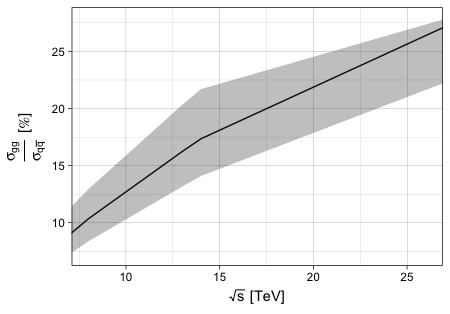
\includegraphics[width=9cm]{./figures/Rplot}
		\caption{The ratio of the LO gluon fusion production cross-section $ gg \to Zh$  ($\sigma_{gg}$) with respect to the NLO Drell-Yan process $ q\bar{q} \to Zh$ cross-section ($\sigma_{q\bar{q}}$) at a $pp$ collider with centre-of-mass energy $\sqrt{s}$. The error band captures the total theoretical uncertainties on both cross-sections dominated by~$\sigma_{gg}$ .}
		\label{fig:hzratio}
	\end{center}
\end{figure}
%%
\par The leading order (LO) contribution to the $g g \rightarrow Z h$ amplitude, given by one-loop diagrams, were computed in refs.\cite{Kniehl:1990iva, Dicus:1988yh}, with full quark mass dependence. For the NLO computations, the virtual corrections contain multi-scale two-loop integrals, some of which are still not known analytically. The first computation of the NLO terms has been accomplished by~\cite{Altenkamp:2012sx}, using the HTL asymptotic expansion and setting $m_b = 0$. The HTL NLO computations pointed to a significant $K$-factor of about $\sim2$.  Later, the computation was improved via soft gluon resummation, including NLL terms found in ref.~\cite{Harlander:2014wda}.  Top quark mass effects were first implemented using a combination of  HTL and Pad\'e approximants~\cite{Hasselhuhn:2016rqt}. A data-driven approach to extract the gluon fusion-dominated non-Drell-Yan part of $Zh$ production using the known relation between  $Wh$
and $ Z h$ associated production has been investigated in ref.~\cite{Harlander:2018yns}. The differential distributions of $g g \rightarrow Zh$  at NLO were studied in ref.~\cite{Hespel:2015zea} via LO matrix element matching. 
%%
\par More recent studies of the NLO virtual corrections to this process were based on the high-energy~(HE) expansion improved by Pad\'e approximants with the LME, which extended the validity range of the HE expansion \cite{Davies:2020drs}. However, this expansion is only valid for in the invariant mass region $\sqrt{\hat{s}}  \gtrsim 750\, \si{\GeV} $ and $\sqrt{\hat{s}}  \lesssim 350\,  \si{\GeV}$ that only covers $\sim 32\%$ of the hadronic cross-section. Furthermore, numerical computation of the two-loop virtual corrections, though implemented exactly in ~\cite{Chen:2020gae}, are rather slow for practical use in MC simulations.  This highlights the importance of an analytical method that can cover the remaining region of the cross-section.  Fortunately, the two-loop corrections to the triangle diagrams can be computed exactly. \\
 In this thesis, I will discuss an approach which allows for an analytic computation of the $gg \to Zh$ process, which covers $95 \%$ of the phase space.  This approach is based on expansion in small  $Z$ (or Higgs) 
 transverse momentum~$\pt$, and was first used for Higgs pair production in~\cite{Bonciani:2018omm} to compute the NLO virtual corrections to the box diagrams in the forward kinematics. While the triangle diagrams are computed exactly. This work, by myself and my collaborators has been published in~\cite{Alasfar:2021ppe}.\\
More recently, the full NLO corrections to this channel has been computed in ref.~\cite{Degrassi2022a}, including the real corrections as well.

\subsection{Associated production with top quarks}
The higher-order corrections to the $t\bar t h /t h$ channel itself, the NLO QCD+EW effects on the off-shell multileptons final state were studied in~\cite{Denner:2019zdz}. In contrast, the NLO corrections, including SMEFT operators, were calculated in\cite{Maltoni:2016yxb}. The NLO QCD+EW with Parton showering is available in all event generators. As of writing this thesis, there is no NNLO calculation of $t\bar t h /t h$ available. 
However, it should be noted that the largest part of the $t\bar t h/th$ expected uncertainty budget comes from the theoretical modelling of this process's backgrounds, mainly $t \bar t b\bar b,\ t\bar t W$ as backgrounds for $ t\bar t (h \to b\bar b)$ and $ t \bar t ( h \to \mathrm{multileptons})$, respectively. There have been several theoretical developments regarding these backgrounds, see for example Refs.~\cite{Broggio:2019ewu,Kulesza:2020nfh,Bevilacqua:2020pzy,Denner:2020hgg,Bevilacqua:2020srb,Denner:2021hqi,Cordero:2021ia,Bevilacqua:2021tzp.Denner:2020orv, Bevilacqua:2021cit}. However,further discussion of the theoretical developments of these channels is beyond the scope of this thesis.


% Starting with $t\bar t W$, the differential cross-section at NNL+ NLO QCD calculation of this channel has been done in~\cite{Broggio:2019ewu,Kulesza:2020nfh} including EW corrections. In addition to the computation of the fully-decayed final state at NLO QCD~\cite{Bevilacqua:2020pzy,Denner:2020hgg,Bevilacqua:2020srb} and at NLO-EW~\cite{Denner:2021hqi}. These calculations were implemented in~\texttt{POWHEG-BOX}~\cite{Cordero:2021iau}. The comparison between the NLO-QCD with Parton showering vs on-shell can be found in~\cite{Bevilacqua:2021tzp}. As for ~$t \bar t b\bar b$, the progress in obtaining higher-order corrections is faced with challenges posed by the complexity of this channel. However, progress has been made. For instance, the off-shell effects in the fully decayed $ pp \to 2 \ell 2 \nu  4 b$ with NLO corrections were studied in~\cite{Denner:2020orv, Bevilacqua:2021cit}. Further discussion of the theoretical developments of these channels is beyond the scope of this thesis. \\

%\section{Higgs pseudo-observables \label{sec:higgspos}  }

\section{Concluding remarks \label{sec:singlehiggsconc}  }
The precision-era of Higgs measurements requires developments on both experimental and theoretical levels. The experimental precision can be improved with higher luminosities and energies, better detectors and improved analysis techniques. Theoretical uncertainties require higher-order calculations in perturbation theory, the inclusion of mixed EW and QCD terms, the inclusion of mass effects and suitable Parton distribution functions at higher order in QCD.  Much effort was and is being put into improving the theoretical predictions of Higgs production channels. Moreover, a plethora of computer tools have been made available to facilitate the computation of these cross-sections, for example  \texttt{iHixs2}~\cite{Dulat:2018rbf} or to generate full events, like \texttt{POWHEG}~\cite{Alioli:2008tz,Nason:2009ai,Bagnaschi:2011tu,Campbell:2012am,Luisoni:2013cuh,Jager:2014vna,Hartanto:2015uka} and \texttt{MadGraph5\_aMC@NLO}~\cite{Alwall:2014hca}. The LHC-Higgs working group is working group that joins the community efforts in making the best predictions available to the theory and experiment community, see their Twiki page for further details~\cite{HXSWG}. 
% \\ Sometimes, to improve the measurement of the process, it is not sufficient to include Higher-order terms of the channel itself and its backgrounds that is particularly important for $t\bar th $. Hence, higher-order calculations of processes like $t\bar t W$ with Parton-shower effects as well as improved analysis to distinguish $t\bar t(h \to b \bar b) $ have a significant impact on~$t\bar th $ measurements.
%Event generator tools with SMEFT implementation for Higgs processes with patron showing interface capabilities have been implemented in a \texttt{MadGraph5\_aMC@NLO} model~\texttt{SMEFTatNLO}~\cite{Degrande:2020evl} that enabled loop computations with SMEFT operators and consequently fits of the SMEFT Wilson coefficients with Higgs data at NLO as we have seen in~\autoref{chap:HiggsEFT}.\\
%There is plenty of room for future improvements in the reduction of theory uncertainty budget and providing better theoretical prediction of the Higgs processes in the SM and beyond, from the inclusion of Patron shower matching, merging and validation to the inclusion of two-loop calculations of gluon fusion $Zh$  and EW NLO effects of  $t\bar the $, all in preparation for the HL-LHC Higgs precision era! 

%%%
%\begin{figure}
%	\begin{center}
	%		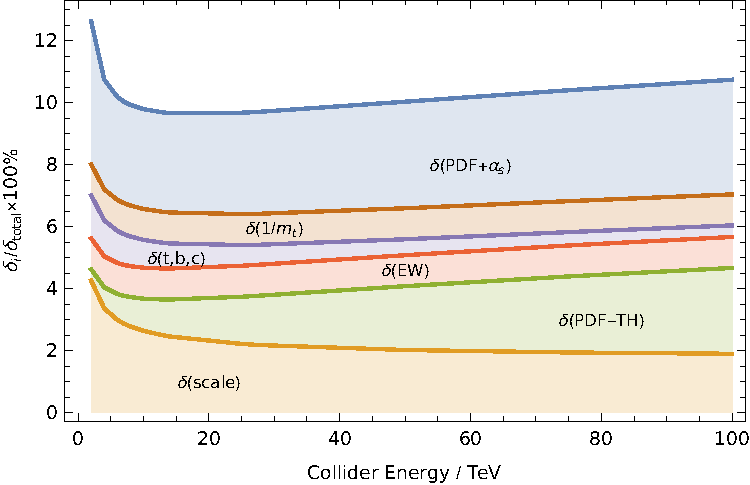
\includegraphics[width=9cm]{./figures/error_plot}
	%		\caption{The error budget plot showing the cumulative uncertainty of the total Higgs cross-section via gluon fusion at ~N$\,^3$LO as a function of energy. This plot is taken from~\cite{Dulat:2018rbf}}
	%		\label{fig:error-budget}
	%	\end{center}
%\end{figure}
%%%


%
%\subsubsection{The LO amplitude}
%We recall the projected LO on shell amplitude~\cite{Gunion:1989we}
%\begin{equation}
%	\mathcal{M}_{LO} = \frac{ T_f \alpha_s \ght }{2 \sqrt{2} \pi } \mathcal F^{(1 \ell)}  S_\epsilon ,
%\end{equation}
%with the projector
%\begin{equation}
%	\mathbb{P}^{\mu \nu} = g^{\mu \nu}- 2\frac{p^\mu_{2} p^\nu }{m_h^2},
%\end{equation}
%and the 1 loop form factor
%\begin{align}
%	\mathcal F^{(1 \ell)} &= m_h\,\sqrt{\tau} \left( (1-\tau) H(0,0,x)+2\right) ,\nonumber  \\
%	x &= \frac{\tau+2 \sqrt{1-\tau}-2}{\tau},
%	\label{f1l}
%\end{align}
%where $ \tau = 4 m_t^2/m_h^2$,  $H(m,n,x)$ is the harmonic ploylogarithm function~(HPL), and
%\begin{equation}
%	S_\epsilon = \Gamma(1+\epsilon) (\mu/m_t)^{2\epsilon}.
%\end{equation}
%\\
%The decay width is therefore given by
%\begin{equation}
%	\Gamma_{LO}(h\to gg) = \frac{\alpha_s^2\, G_F\,m_h^3 \,m_t^2\,\tau }{8 \pi^3 \sqrt{2}}  \, \left( 3(\tau-1)^2 H(0,0,0,0,x)+2(\tau-1)H(0,0,x)+2\right)
%\end{equation}
%With the following definitions
%\begin{align}
%	\ght &=\ght^{SM} = {\sqrt{2} m_t \over v}, \nonumber \\
%	v &= \left( G_F \sqrt{2}\right) ^{-1/2}, \nonumber \\
%	T_f &= \frac{1}{2} .
%\end{align}